\documentclass{anstrans}
%%%%%%%%%%%%%%%%%%%%%%%%%%%%%%%%%%%
\title{Comparison Between Gaussian Processes and DMD Surrogates for Isotopic Composition Prediction}
\author{Rabab Elzohery, Mohammad Abdo, and Jeremy Roberts}

\institute{
Department of Mechanical \& Nuclear Engineering, Kansas State University, Manhattan, KS 66506
}

% Optional disclaimer: remove this command to hide
%\disclaimer{Notice: this manuscript is a work 4of fiction. Any resemblance to
%actual articles, living or dead, is purely coincidental.}

%%%% packages and definitions (optional)
\usepackage{graphicx} % allows inclusion of graphics
\usepackage{booktabs} % nice rules (thick lines) for tables
\usepackage{microtype} % improves typography for PDF
\usepackage{lipsum}

\newcommand{\SN}{S$_N$}
\renewcommand{\vec}[1]{\bm{#1}} %vector is bold italic
\newcommand{\vd}{\bm{\cdot}} % slightly bold vector dot
\newcommand{\grad}{\vec{\nabla}} % gradient
\newcommand{\ud}{\mathop{}\!\mathrm{d}} % upright derivative symbol

\begin{document}
%%%%%%%%%%%%%%%%%%%%%%%%%%%%%%%%%%%%%%%%%%%%%%%%%%%%%%%%%%%%%%%%%%%%%%%%%%%%%%%%
\section{Introduction}

The next frontier of reactor modeling will require large-scale, full-core, transient models.
However, the herculean efforts involved will not likely be feasible for applications in which a system model must be executed for multiple system perturbations, e.g., design optimization and uncertainty quantification.
Hence, relatively  inexpensive surrogate models may be needed.

Given access to a high-fidelity model and corresponding solution, data-driven techniques can be used to generate surrogates without resorting to simplified physics or modifying the underlying implementation.  
One class of surrogates recently explored in the nuclear engineering community are those based on dynamic-mode decomposition \cite{}.  
These past applications involved spatiotemporal dynamics that evolved relatively slowly in time, e.g., the evolution of isotopics \cite{} and decay-heat generation \cite{}.

Reactor transients exhibit much different dynamics.
With the restart of TREAT, preliminary efforts to apply generate surrogates based on gPC for uncertainty quantification have had some success \cite{}.
However, the surrogates generated lacked explicit time dependence and required substantial user development.

Presented here is the development of a data-driven surrogate based on dynamic-mode decomposition (DMD) to approximate time- and space-dependent fluxes and powers.
Specifically, a surrogate was produced for the 2-D LRA transient diffusion benchmark to illustrate the potential of the DMD approach. 
Whereas a conventional DMD surrogate cannot capture the rapid dynamics of the LRA transient, a sequence of DMD surrogates defined for successive time windows proved more effective, the details of which are presented below.


%%%%%%%%%%%%%%%%%%%%%%%%%%%%%%%%%%%%%%%%%%%%%%%%%%%%%%%%%%%%%%%%%%%%%%%%%%%%%%%%
\section{Theory}
\subsection{Gaussian Process Based Surrogate}
The first method applied in this work is the Gaussian Process (GP) regression \cite{eldred2006dakota}. Gaussian Process (a.k.a, Kriging) is a surface fitting  method used to build an approximate function given a set of training points generated by the original model. It provides the predictions and their associated uncertainties at unknown points.
The GP emulator at any point $\mathbf{x}$ has the form:
\begin{equation}
f^{\mathcal{GP}}(\mathbf{x}) = \mathbf{g}(\mathbf{x})^T\boldsymbol{\beta} + \mathbf{k}(\mathbf{x})^T\mathbf{K}^{-1}(\mathbf{f}-\mathbf{G}\boldsymbol{\beta}),
\end{equation}
where $\mathbf{g}(\mathbf{x})^T\boldsymbol{\beta}$ is the hypothesis (trend) function whose vector of regression coefficients $\boldsymbol{\beta}$ is a least-squares fit of the data, $\mathbf{k}(\mathbf{x})$ is the correlation vector between current $\mathbf{x}$ and the data points, $\mathbf{f}$ is the vector of responses of the high fidelity code under inspection, and $\mathbf{G}$ contains the evaluation of the trend basis functions at all data points. The symmetric matrix $\mathbf{K}$ is the correlation matrix of all data defined as, 
\begin{equation}
\label{eq:Kij}
\mathbf{K}_{i,j}=k(\mathbf{X}_i,\mathbf{X}_j)=exp(-\sum_{k=1}^{m}\theta_k|\mathbf{X}_{i,k}-\mathbf{X}_{j,k}|^\gamma),
\end{equation}
% , $r$ is  determined by an assumed correlation between point $x$ and all the data point where R is a correlation matrix between the data points.
% The Gaussian correlation function is commonly used in GP surrogates:
% \begin{equation}
% r(x, x\prime) = exp(-\sum_{k=1}^{m}\theta_k|X_{i,k}-X_{j,k}|^\gamma)
% \end{equation}
where $\gamma$ and $\theta$'s are hyper parameters that are computed via Maximum Likelihood Estimation (MLE). Equation \ref{eq:Kij} is interchangeably referred to as the powered-exponential covariance (kernel or correlation) function. 

Construction of a surrogate model with a relatively high-dimensional input/output space may be prohibitively expensive. Rather a dimensionality reduction technique can be used with the surrogate when the data has a potential for reduction. In this work, both the inputs and outputs are the isotopic compositions, and it is desired to track a large number of isotopes with sufficient spatial resolution which increases the problem space. Also, strong correlations exist between the different isotopic concentrations and hence it should be possible to apply a dimension reduction method in conjunction with the surrogate.

One reduction method that is commonly used with GP  is Principal Component Analysis (PCA).  The basic idea of PCA relies on the transform of the basis on which the data is represented. In other words, the data will be re-expressed in terms of a different coordinate system that better explains the variance of the data. 
Consider a data matrix $\mathbf{X}\in \mathbb{R}^{n\times m}$, where $n$ is the dimension of the feature space and $m$ is the number of snapshots, new orthonormal basis can be identified by computing the Singular Value Decomposition (SVD) of this data matrix, i.e,
\begin{equation}\label{svd}
 {\mathbf{X = U\Sigma V}}^H,
 \end{equation}
where \textbf{U} is a unitary matrix whose columns span the new space onto which the data are projected, $\boldsymbol{\Sigma}$ is a diagonal matrix containing the singular values, which can be interpreted as the variance of the data along the corresponding left singular vector, \textbf{V} is the right singular matrix, and $(.)^{H}$ denotes the hermitian conjugate.
Assuming the data has a potential of reduction, the first $r$ vectors are used to construct an active subspace onto which the data will be projected.
The  decorrelated reduced basis can now be re-expressed as a linear combination of the original basis, each weighted according to its contribution to the data variance. A surrogate model can then be trained using data  mapped from the projected  data $X^{(r)}$,
\begin{equation}
\mathbf{X}^{(r)} = \mathbf{U}_r ^T \mathbf{X}.
\end{equation}
In this study, the DAKOTA framework was used to build the GP surrogate \cite{eldred2006dakota}.
\subsection*{Dynamic Mode Decomposition}
Dynamic Mode Decomposition (DMD) is a model decomposition that can serve as another ROM technique. DMD is an emerging tool that has been used recently for analyzing the behavior of dynamic systems. It is capable of providing a spatio-temporal decomposition of the data of interest into the dominant dynamic modes, i.e, DMD modes, using a set of data snapshots.
Consider the same data matrix in the previous subsection $\textbf{X}$, but now splitting it into two data matrices, whose columns represent snapshots equally spaced by a step $\Delta t$ as follows,
\begin{subequations}
\begin{equation}
	\mathbf{X_1}=\left[\begin{array}{cccc}
	| & | &    | \\ 
	{\mathbf{x_1}} &   ... & {\mathbf{x_{m-1}}} \\ 
	| & | &  |
	\end{array} \right]\, 
   \end{equation}
    \begin{equation}
	{\mathbf{X_2}}=\left[\begin{array}{ccc}
	| & | &   | \\ 
	{\mathbf{x_2}} &  ... & {\mathbf{x_{m}}} \\ 
    | & | &   |
	\end{array} \right] 
    \end{equation}
    \end{subequations}
 The basic assumption here is that there is a linear operator $\textbf{A}$ that approximates the dynamic behavior of the system  such that
\begin{equation}
\mathbf{X_2} \approx \mathbf{A X_1}.
 \end{equation}
 The problem now reduces to finding the eigenpairs of the operator $\textbf{A}$. As a first step,  the PCA modes need to be estimated in a way similar to what has been discussed above.
By using those PCA modes, an approximation of the operator $\textbf{A}$ can be defined as
 \begin{equation}
 \mathbf{\tilde{A} = U_r^{H} A U_r}.
 \end{equation}
 Since the matrix $\tilde{A}$ is related to $A$ via a similarity transformation, they have a common set of eigenvalues, which can be found by evaluating the eigenvalue decompositions
 \begin{equation}\label{eigenvalue}
 \mathbf{\tilde{A} W}=\mathbf{W \Lambda}.
 \end{equation}
The DMD modes can then be expressed as
\begin {equation}
{\mathbf{\Phi}}^{DMD}={\mathbf{X_2V_r\Sigma_r^{-1}W}}.
\end{equation}
Finally, the predicted response at any time is
\begin{equation}
\mathbf{X}^{DMD}(t)=\sum_{i=1}^{r} b_i \mathbf{\phi}_i^{DMD} e^{w_it}={\mathbf{\Phi}}^{DMD}{\mathbf{diag}}(e^{\mathbf{w}t})\mathbf{b},
\end{equation}
where $\textbf{b}$ is the amplitude of the initial condition projected on the DMD modes, and $w_i$ is the discrete characterization of the continuous eigen values computed in \eqref{eigenvalue}.
\begin{equation}
w_i=log(\lambda_i)/\Delta t,
\end{equation}
where $\lambda_i$ is the $i^{th}$ diagonal element in $\boldsymbol{\Lambda}$.



\section{Numerical Experiments and Results}
%%%%%%%%%%%%%%%%%%%%%%%%%%%%%%%%%%%%%%%%%%%%%%%%%%%%%%%%%%%%%%%%%%%%%%%%%%%%%%%%
To examine the two methods demonstrated above, two numerical experiments were conducted in which a standard TRIGA fuel element placed in a square-pitch cell was depleted using Serpent to provide training data for  surrogate construction and  testing points to assess their predictions. The fuel element was discretized axially into three equal segments. A total of 61 isotopes were tracked, leading to a 183-dimensional space.

\subsection{Case study 1}
The first case study depleted a fresh TRIGA fuel element at 600$^{\circ}$ K to 55 GWD/MTHM which is approximately the highest burnup of all the fuel elements in the KSU core.  A total of 150 snapshots were produced, of which 75  were used for training and 75 were used for testing.
By inspecting the singular values computed by \eqref{svd} and shown in Fig\ref{fig:svd}, it was inferred that 3 dimensional subspace would be sufficient to capture most of the data variance.
\begin{figure}[!htb] 
  \centering
  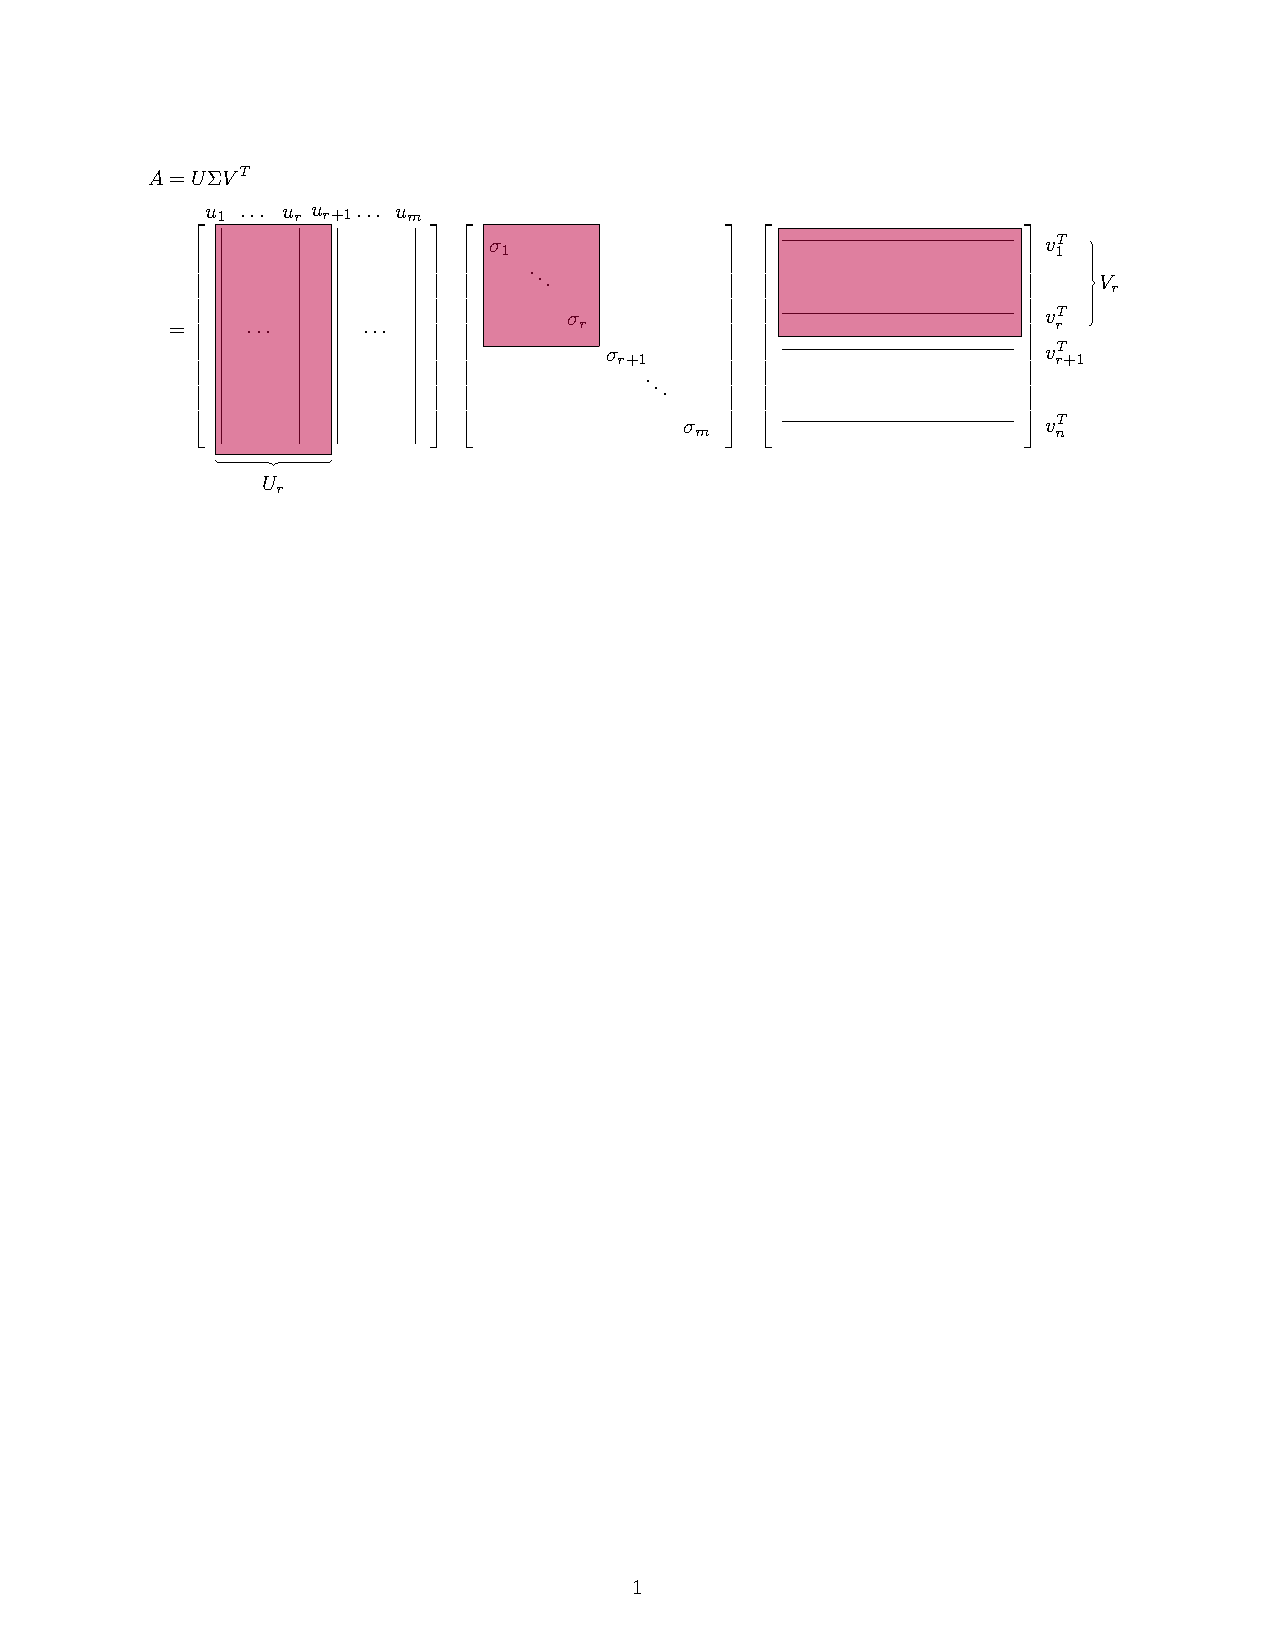
\includegraphics[scale=0.5]{./figures/svd.png}
  \caption{Singular Values.}
  \label{fig:svd}
\end{figure}
To compare the two surrogates and assess their performance, the relative errors in their predictions were estimated for all of the isotopic compositions involved in the study, but results for only ${}^{238}$U, ${}^{239}$Pu, ${}^{235}$U, ${}^{137}$Cs and ${}^{241}$Am of one segment are shown here for brevity.
As shown in figs \ref{u235_err1} and \ref{u238_err1}, both methods were able to predict the compositions of ${}^{238}$U and ${}^{235}$U with a reasonable accuracy,i.e, the maximum relative error in ${}^{235}$U predictions are $0.0175\%$ and $0.0258\%$ for GP and DMD surrogates respectively, while for ${}^{238}$U, the errors are $0.00023\%$ and $0.0026\%$. 
For the other nuclides shown in figs \ref{pu239_err1} through \ref{Cs137_err1}, neither method offered good predictions at early irradiation times, and this was also the case for most of the nuclides that were present with low concentrations at the beginning of the irradiation history. The predictions of both surrogates improved for later times, which indicates that the surrogates treated those isotopes as a background at the beginning since they did not contribute much to the dynamics because of their minor concentrations which in turn made their representations in the leading vectors computed by the SVD weak, but as soon as they start to evolve and make contribution, the surrogates were able recognize their presence and gave better predictions.
In case of DMD, the predicted isotopic compositions were then used to estimate the corresponding $k$-eigenvalue in order to assess the predictions based on a more global quantity. It was found that the maximum observed reactivity bias is about 0.1\%,i.e,  less than \$ 1.00 of reactivity. 
\begin{figure}[!htb] 
  \centering
  \includegraphics[scale=0.5]{./figures/error_U235_case1.png}
  \caption{Relative Errors in ${}^{235}$U.}
  \label{u235_err1}
\end{figure}
\begin{figure}[!htb] 
  \centering
  \includegraphics[scale=0.5]{./figures/error_U238_case1.png}
  \caption{Relative Errors in ${}^{238}$U.}
  \label{u238_err1}
\end{figure}
\begin{figure}[!htb] 
  \centering
  \includegraphics[scale=0.5]{./figures/error_Pu239_case1.png}
  \caption{Relative Errors in ${}^{239}$Pu.}
  \label{pu239_err1}
  \end{figure}
  \begin{figure}[!htb] 
  \centering
  \includegraphics[scale=0.5]{./figures/error_Am241_case1.png}
  \caption{Relative Errors in ${}^{241}$Am.}
  \label{Am241_err1}
\end{figure}
\begin{figure}[!htb] 
  \centering
  \includegraphics[scale=0.5]{./figures/error_Cs137_case1.png}
  \caption{Relative Errors in ${}^{137}$Cs.}
  \label{Cs137_err1}
\end{figure}
%  \begin{figure}[htbp]
% \begin{minipage}[t]{0.5\linewidth}
%     \includegraphics[width=\linewidth, height=3.5cm]{./figures/value_U235_case1.png}
%     \caption{${}^{235}$U Concentration }
%     \label{u235_value1}
% \end{minipage}%
%     \hfill%
% \begin{minipage}[t]{0.5\linewidth}
%     \includegraphics[width=\linewidth, height=3.5cm]{./figures/error_U235_case1.png}
%     \caption{Relative Errors in ${}^{235}$U}
%     \label{u235_err1}
% \end{minipage} 
% \end{figure}
%  \begin{figure}[htbp]
% \begin{minipage}[t]{0.5\linewidth}
%     \includegraphics[width=\linewidth, height=3.5cm]{./figures/value_U238_case1.png}
%     \caption{${}^{238}$U Concentration}
%     \label{u238_valu1}
% \end{minipage}%
%     \hfill%
% \begin{minipage}[t]{0.5\linewidth}
%     \includegraphics[width=\linewidth, height=3.5cm]{./figures/error_U238_case1.png}
%     \caption{Relative Errors in ${}^{238}$U}
%     \label{u238_err1}
% \end{minipage} 
%\end{figure}
% \begin{figure}[htbp]
% \begin{minipage}[t]{0.5\linewidth}
%     \includegraphics[width=\linewidth, height=3.5cm]{./figures/value_Pu239_case1.png}
%     \caption{{${}^{239}$Pu Concentration}}
%     \label{pu239_value1}
% \end{minipage}%
%     \hfill%
% \begin{minipage}[t]{0.5\linewidth}
%     \includegraphics[width=\linewidth, height=3.5cm]{./figures/error_Pu239_case1.png}
%     \caption{Relative Errors in ${}^{239}$Pu}
%     \label{pu239_err1}
% \end{minipage} 
% \end{figure}
% \begin{figure}[htbp]
% \begin{minipage}[t]{0.5\linewidth}
%     \includegraphics[width=\linewidth, height=3.5cm]{./figures/value_Cs137_case1.png}
%     \caption{${}^{137}$Cs Concentration}
%     \label{cs137_valu1}
% \end{minipage}%
%     \hfill%
% \begin{minipage}[t]{0.5\linewidth}
%     \includegraphics[width=\linewidth, height=3.5cm]{./figures/error_Cs137_case1.png}
%     \caption{Relative Errors in ${}^{137}$Cs}
%     \label{cs137_err1}
% \end{minipage} 
% \end{figure}
% \begin{figure}[htbp]
% \begin{minipage}[t]{0.5\linewidth}
%     \includegraphics[width=\linewidth, height=3.5cm]{./figures/value_Am241_case1.png}
%     \caption{{${}^{241}$Am Concentration}}
%     \label{am241_value1}
% \end{minipage}%
%     \hfill%
% \begin{minipage}[t]{0.5\linewidth}
%     \includegraphics[width=\linewidth, height=3.5cm]{./figures/error_Am241_case1.png}
%     \caption{Relative Errors in ${}^{241}$Am}
%     \label{am241_err1}
% \end{minipage} 
% \end{figure}



\subsection{Case study 2}
To examine the performance of the two surrogates more thoroughly, another case with a perturbed initial condition was studied. Here, the fuel was depleted to 25 GWD/MTHM under an elevated temperature of 800$^{\circ}$K  and then depleted another 10 GWD/MTHM at 600 $^{\circ}$K, which is similar to what happens when a hot element is shuffled to another location at lower temperature inside the reactor core. This could introduce a nonlinear effect and hence, produce nuclide concentrations that deviate from the original training domain. 
For this case study, the GP surrogate was trained using the same dataset used in the previous study, and for DMD, the eigenpairs are the ones obtained using this dataset, too. 
The figures below show that DMD outperforms GP. This is not surprising since DMD is a physics revealing technique that provides the spatial-temporal modes which demonstrate the physical state of the system so they can  still be representative of the perturbed system to some extent, while the GP method used here is an interpolation method that performs well if the unknown points lie inside the training domain but performs poorly  if the points deviate from this space. 


 \begin{figure}[!htb] 
  \centering
  \includegraphics[scale=0.5]{./figures/error_U235_case2.png}
  \caption{Relative Errors in ${}^{235}$U.}
  \label{u235_err2}
\end{figure}
\begin{figure}[!htb] 
  \centering
  \includegraphics[scale=0.5]{./figures/error_U238_case2.png}
  \caption{Relative Errors in ${}^{238}$U.}
  \label{u238_err2}
\end{figure}
\begin{figure}[!htb] 
  \centering
  \includegraphics[scale=0.5]{./figures/error_Pu239_case2.png}
  \caption{Relative Errors in ${}^{239}$Pu.}
  \label{u239_err2}
  \end{figure}
%   \begin{figure}[!htb] 
%   \centering
%   \includegraphics[scale=0.5]{./figures/error_Am241_case2.png}
%   \caption{Relative Errors in ${}^{241}$Am.}
%   \label{Am241_err2}
% \end{figure}
\begin{figure}[!htb] 
  \centering
  \includegraphics[scale=0.5]{./figures/error_Cs137_case2.png}
  \caption{Relative Errors in ${}^{137}$Cs.}
  \label{Cs137_err2}
\end{figure}


 The reactivity bias resulting from the DMD predictions was found to be no larger than 0.2\%.
\subsection{Conclusion}
GP and DMD are two reduced-order models that were used here  to predict the isotopic compositions of a TRIGA fuel element at different burnups.
It was shown that both methods perform well when the desired prediction lies inside the space used to train the surrogates. When a perturbation was introduced to the system, DMD  was still able to provide  an acceptable prediction. However, GP failed, and there was a noticeable difference in its performance compared to the original case.
It is expected that the GP surrogate would be improved by widening the sampling space to include more snapshots from several perturbed cases. However, improvement in DMD could be introduced without requiring more computational burden  by using more advanced DMD algorithm such as Multi-Resolution DMD and optimized Koopman DMD.
Future work will include an extension of these methods to  
a full TRIGA core and relate uncertainty and sensitivity analysis.
%Also, It is important to mention that where the number of snapshots is a critical ingredient that affects the quality of GP surrogates, i.e; increasing the number of snapshots enhances the quality of the surrogate, this is not the case In DMD. This can be proved by 



\section{Acknowledgments}
The material \cite{bowman2011scale} presented is based on work supported in part by the U.S. Nuclear Regulatory Commission, Office of Nuclear Regulatory Research, under award number NRC-HQ-60-15-G-0004.
%%%%%%%%%%%%%%%%%%%%%%%%%%%%%%%%%%%%%%%%%%%%%%%%%%%%%%%%%%%%%%%%%%%%%%%%%%%%%%%%
\bibliographystyle{ans}
\bibliography{bibliography}
\end{document}

